The magnetic field $\boldsymbol{B_p}$ of a mobile device without iron effects can be described with roll $\phi$, pitch $\theta$ and $\psi$ as the equation:
\begin{equation} \label{eq:magnField}
  \boldsymbol{B_p} = 
  \boldsymbol{R_x}(\phi)\boldsymbol{R_y}(\theta)\boldsymbol{R_z}(\psi)\boldsymbol{B_r} = 
  \boldsymbol{R_x}(\phi)\boldsymbol{R_y}(\theta)\boldsymbol{R_z}(\psi)B\begin{pmatrix}cos(\delta) \\ 0  \\ sin(\delta)\end{pmatrix}
\end{equation}
with the rotations where $ \boldsymbol{R_x}(\phi)$,$\boldsymbol{R_y}(\theta)$ and $\boldsymbol{R_z}(\psi)$ is the rotation matrices, $\boldsymbol{B_r}$ is the local geomagnetic field vector with magnitude $B$ and the magnetic tilt $\delta$. The hard iron offset can be described as the vector $\boldsymbol{V_{PCB}}$ which will according to ~\cite{sensor:magnIron} appear additive to the vector of the sensor $\boldsymbol{V_{Sensor}}$. This gives the equation:
\begin{equation}
\end{equation}
~\cite[]{sensor:magnIron}

  When looking at devices with similar or same hardware you can see differences in measurements, for example here are the accelerometer recordings from 5 iPhone 6 and 1 iPhone 5S:
\begin{figure}[H]
\centering
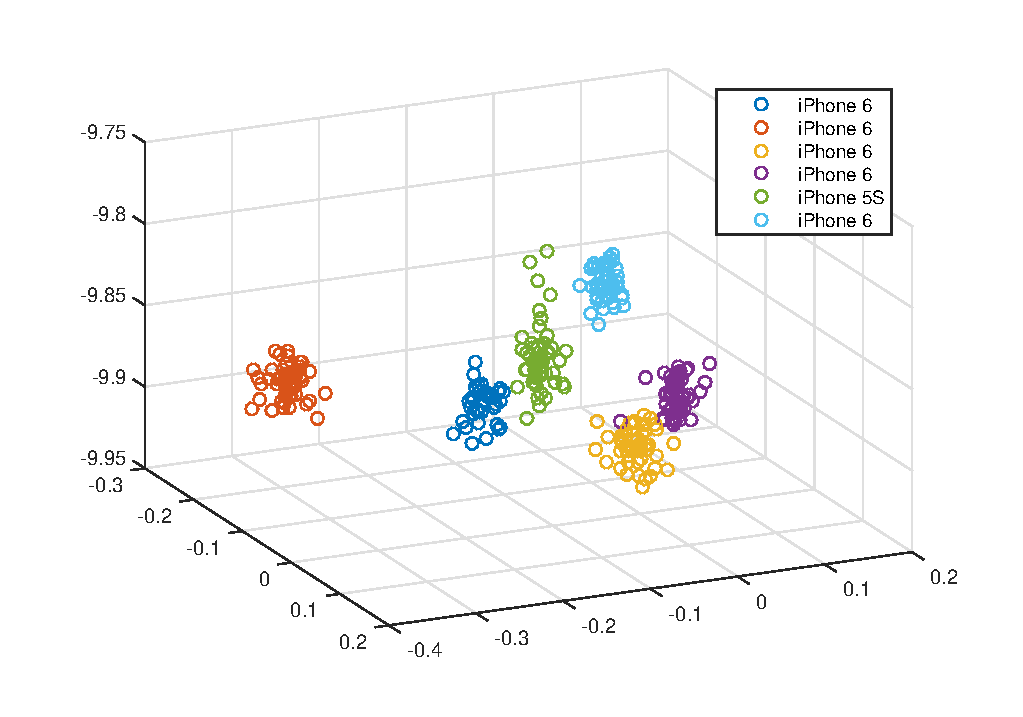
\includegraphics[scale=.6]{img/scatteriPhone}
\caption{Scatter graph on accelerometer recordings of 6 Apple devices}
\label{fig:digraph}
\end{figure}

\section{Magnetometer\index{magnetometer}}
The magnetometer measures the magnetic field and was originally used for navigation and tracking. When it is used as a compass the Earth's magnetic field is measured. The type of sensor found in mobile devices is like accelerometer and gyroscope a MEMS sensor. They are known as e-compasses gaussmeters that is measuring of magnetic fields larger than 1 nT.
~\cite[]{sensor:magn}

\subsection{Fingerprinting feature / Bias}
\textit{Note that normally bias in a magnetometer is called \textbf{offset} but for uniformity reason of this report it will be referenced to \textbf{bias}.}\\
\\
When try to measure the magnetic field of Earth with a magnetometer it also gets affected by other magnetic fields. The two main error sources from measurements of magnetometer are magnetic contamination in the sensor, called Soft and Hard-Iron distortion. \\
The hard iron distortion is caused by metals and magnets around the magnetometer. This field is constant even if the device moves, thus it is additive to the earths magnetic field. This distortion can be caused of e.g. the device speaker mounted near the magnetometer. \\
If there are magnetic fields in the surrounding environment of the device they will cause soft iron disorder. This error is smaller than the hard iron distortion. Any metal around the device can cause this error, such a car passing by.
There are also a third bias that can effect the magnetometer and is as the hard iron distortion additive. This bias is the errors in the magnetometer itself such that all hardware has. But the result of this bias is similar to the soft iron distortion.  \\
The good thing with magnetometer bias is that it is constant over time, thus once it is calculated it stays the same. \\
\\
If the device is rotated one turn (360\degree)around its own z-axes (see~\figureref{fig:device-axes}) and plot x with respect to y there will be a circle. In a world without bias this circle will look like:
\begin{figure}[H]
\begin{tabular}{p{0.23\textwidth} p{0.23\textwidth} p{0.23\textwidth} p{0.23\textwidth}}
        \vspace{0pt} \begin{tikzpicture}[line cap=round,line join=round,>=triangle 45,x=1.0cm,y=1.0cm]
\draw[->,color=black] (-1.5,0.) -- (1.5,0.);
\foreach \x in {-1.4,-1.2,-1.,-0.8,-0.6,-0.4,-0.2,0.2,0.4,0.6,0.8,1.,1.2,1.4}
\draw[shift={(\x,0)},color=black] (0pt,-2pt);
\draw[color=black] (1.3548383992423667,0.012646598999199708) node [anchor=south west] {X};
\draw[->,color=black] (0.,-1.5) -- (0.,1.5);
\foreach \y in {-1.4,-1.2,-1.,-0.8,-0.6,-0.4,-0.2,0.2,0.4,0.6,0.8,1.,1.2,1.4}
\draw[shift={(0,\y)},color=black] (-2pt,0pt);
\draw[color=black] (0.015808248748999637,1.4306334471160802) node [anchor=west] {Y};
\clip(-1.5,-1.5) rectangle (1.5,1.5);
\draw(0.,0.) circle (1.cm);
\begin{scriptsize}
\draw [color=xdxdff] (0.,0.)-- ++(-2.0pt,-2.0pt) -- ++(4.0pt,4.0pt) ++(-4.0pt,0) -- ++(4.0pt,-4.0pt);
\draw [fill=qqqqff] (0.,1.) circle (1.5pt);
\draw[color=qqqqff] (-0.15,1.1) node {0\textrm{\degre}};
\end{scriptsize}
\end{tikzpicture}
 & 
        \vspace{0pt} \begin{tikzpicture}[line cap=round,line join=round,>=triangle 45,x=1.0cm,y=1.0cm]
\draw[->,color=black] (-1.5,0.) -- (1.5,0.);
\foreach \x in {-1.4,-1.2,-1.,-0.8,-0.6,-0.4,-0.2,0.2,0.4,0.6,0.8,1.,1.2,1.4}
\draw[shift={(\x,0)},color=black] (0pt,-2pt);
\draw[color=black] (1.3548383992423672,0.012646598999199708) node [anchor=south west] {X};
\draw[->,color=black] (0.,-1.5) -- (0.,1.5);
\foreach \y in {-1.4,-1.2,-1.,-0.8,-0.6,-0.4,-0.2,0.2,0.4,0.6,0.8,1.,1.2,1.4}
\draw[shift={(0,\y)},color=black] (-2pt,0pt);
\draw[color=black] (0.015808248748999637,1.4306334471160802) node [anchor=west] {Y};
\clip(-1.5,-1.5) rectangle (1.5,1.5);
\draw(-0.2,-0.2) circle (1.003958800671448cm);
\begin{scriptsize}
\draw [fill=qqqqff] (-0.18558461983368865,0.8038553034478191) circle (1.5pt);
\draw[color=qqqqff] (-0.16,1) node {0\textrm{\degre}};
\draw [color=xdxdff] (-0.2,-0.2)-- ++(-2.0pt,-2.0pt) -- ++(4.0pt,4.0pt) ++(-4.0pt,0) -- ++(4.0pt,-4.0pt);
\end{scriptsize}
\end{tikzpicture} & 
        \vspace{0pt} \begin{tikzpicture}[line cap=round,line join=round,>=triangle 45,x=1.0cm,y=1.0cm]
\draw[->,color=black] (-1.5002742877331638,0.) -- (1.5002742877331638,0.);
\foreach \x in {-1.4,-1.2,-1.,-0.8,-0.6,-0.4,-0.2,0.2,0.4,0.6,0.8,1.,1.2,1.4}
\draw[shift={(\x,0)},color=black] (0pt,-2pt);
\draw[color=black] (1.3548383992423672,0.012646598999199708) node [anchor=south west] {X};
\draw[->,color=black] (0.,-1.500215870948452) -- (0.,1.5001897416116785);
\foreach \y in {-1.4,-1.2,-1.,-0.8,-0.6,-0.4,-0.2,0.2,0.4,0.6,0.8,1.,1.2,1.4}
\draw[shift={(0,\y)},color=black] (-2pt,0pt);
\draw[color=black] (0.015808248748999637,1.4306334471160802) node [anchor=west] {Y};
\clip(-1.5002742877331638,-1.500215870948452) rectangle (1.5002742877331638,1.5001897416116785);
\draw [rotate around={-36.86989764584405:(0.,-0.15)}] (0.,-0.15) ellipse (1.1608455676650522cm and 0.8860374890305703cm);
\begin{scriptsize}
\draw [color=xdxdff] (0.04907705257499707,-0.12173658003568395)-- ++(-2.0pt,-2.0pt) -- ++(4.0pt,4.0pt) ++(-4.0pt,0) -- ++(4.0pt,-4.0pt);
\draw [fill=qqqqff] (-0.8962562226151813,0.5864729639194997) circle (1.5pt);
\draw[color=qqqqff] (-1.1,0.75) node {0\textrm{\degre}};
\end{scriptsize}
\end{tikzpicture} & 
        \vspace{0pt} \begin{tikzpicture}[line cap=round,line join=round,>=triangle 45,x=1.0cm,y=1.0cm]
\draw[->,color=black] (-1.500130470417328,0.) -- (1.5002743955178048,0.);
\foreach \x in {-1.4,-1.2,-1.,-0.8,-0.6,-0.4,-0.2,0.2,0.4,0.6,0.8,1.,1.2,1.4}
\draw[shift={(\x,0)},color=black] (0pt,-2pt);
\draw[color=black] (1.3548385432174719,0.012646598999199708) node [anchor=south west] {X};
\draw[->,color=black] (0.,-1.500215870948452) -- (0.,1.5001897416116785);
\foreach \y in {-1.4,-1.2,-1.,-0.8,-0.6,-0.4,-0.2,0.2,0.4,0.6,0.8,1.,1.2,1.4}
\draw[shift={(0,\y)},color=black]  (-2pt,0pt);
\draw[color=black] (0.015808244815253596,1.4306334471160802) node [anchor=west] {Y};
\clip(-1.500130470417328,-1.500215870948452) rectangle (1.5002743955178048,1.5001897416116785);
\draw [rotate around={0.059845574260994405:(4.8164851529053886E-4,7.838801032565946E-4)}] (4.8164851529053886E-4,7.838801032565946E-4) ellipse (1.2496624710485813cm and 0.9992161789727994cm);
\begin{scriptsize}
\draw [color=xdxdff] (0.,0.)-- ++(-2.0pt,-2.0pt) -- ++(4.0pt,4.0pt) ++(-4.0pt,0) -- ++(4.0pt,-4.0pt);
\draw [fill=qqqqff] (0.,1.) circle (1.5pt);
\draw[color=qqqqff] (-0.15,1.1) node {0\textrm{\degre}};
\end{scriptsize}
\end{tikzpicture} \\
        \vspace{0pt} Ideal & Hard Iron distortion & Soft Iron distortion & Gain mismatch \\
\end{tabular}
\caption{Example of different magnetometer readings when affected by bias.}\label{fig:magnCircle}
\end{figure}
\cite[]{liu:magnAcc}

\subsection{Magnetometer calibration}
To do a magnetometer calibration the device is turned 360\degree around the z-axis (~\figureref{fig:device-axes}), with the device on a flat surface. This makes x and y-axis the surface and z-axis pointing (UP/DOWN?). To calculate the offset $O_{x,y,z}$ the average of min and max-value from each axis is calculated (the center of the circle) from the magnetic field $B_{x,y,z}$, like:
\begin{subequations}
\begin{align}
  O_x = \frac{max(B_x) + min(B_x)}{2} \\
  O_y = \frac{max(B_y) + min(B_y)}{2} \\
  O_z = \frac{max(B_z) + min(B_z)}{2}
\end{align} 
And the hard iron compensated result $m_{x,y,z}^h$:
\begin{align}
  m_x^h = B_x - O_x \\
  m_y^h = B_y - O_y \\
  m_z^h = B_z - O_z
\end{align}
\end{subequations}
The soft iron is sometimes compensated for in the equations above and sometimes additional compensation has to be done. Since soft iron offset is place specific it will not be considered in the thesis since a fingerprint of a device is not convenient if you have to be at the exact same spot every time the device tries to authenticate.
\cite[]{liu:magnAcc}